% Carried over verbatim from monograph/main.tex (Study 1 record, 13 Sep 2026).
\chapter{Reproduction and release engineering}\label{s1:ch:ch16_reproduction_and_release_engineering}

\section{From owner downloads to structural Table 1}

\begin{figure}[H]
\centering
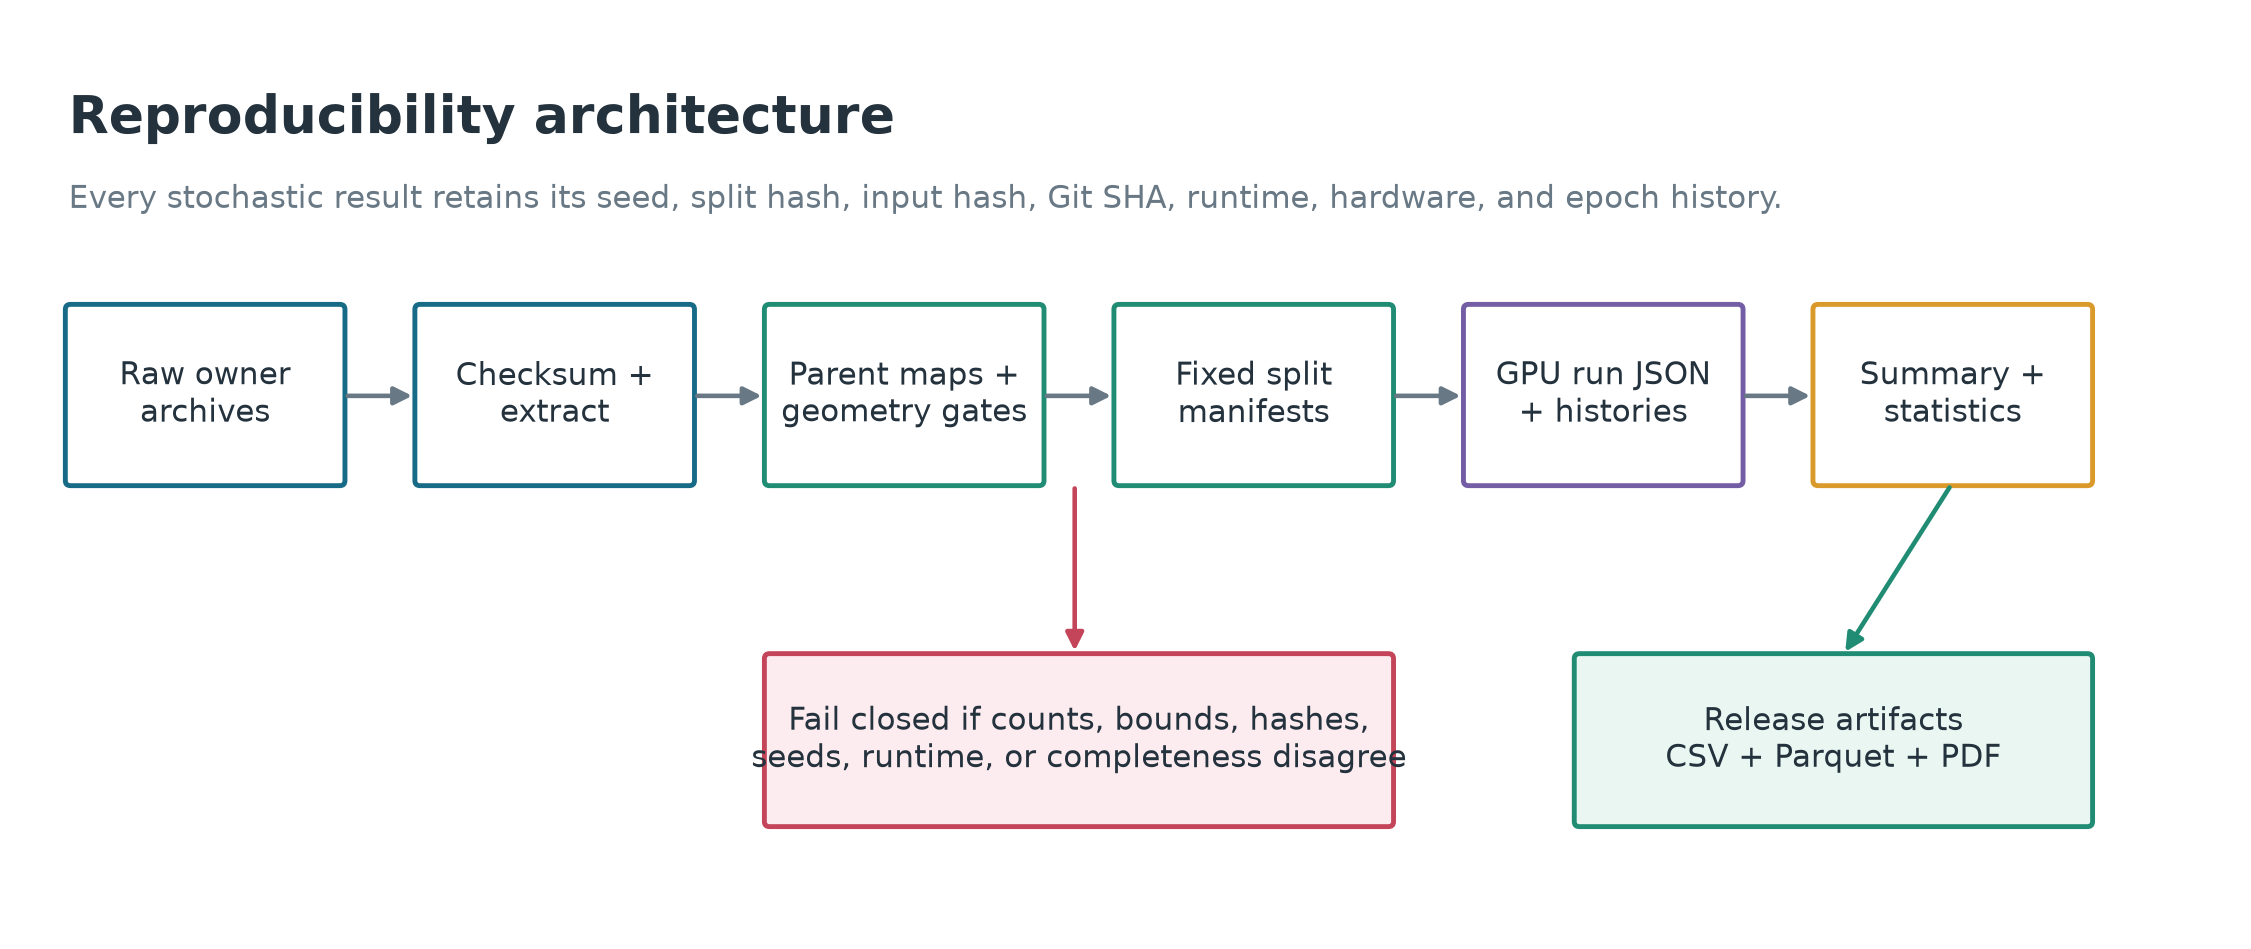
\includegraphics[width=\textwidth]{reproducibility_pipeline.png}
\caption{The intended clean-clone path. Each boundary writes an auditable artifact and performs validation before the next stage begins.}
\label{s1:fig:reproduction}
\end{figure}

The GPU-free structural result has one public entry point:
\begin{lstlisting}[style=cyto,language=bash,caption={Raw-download-to-Table-1 entry point.}]
./scripts/reproduce_table1.sh
\end{lstlisting}
The script performs a locked dependency sync; downloads all declared owner files with at most three connections; verifies exact sizes and SHA-256 values; extracts archives; recovers SIPaKMeD, Cx22, CRIC, and Herlev provenance; runs the SIPaKMeD duplicate and pixel-overlap audits; creates fixed splits; and emits the dataset-level and seed-level structural tables.

Raw images are intentionally excluded from version control. The repository distributes URLs, checksums, IDs, coordinates, derived maps, split assignments, and results, subject to each source's terms. In particular, Cx22/CCEDD assets are non-commercial research resources and are not repackaged in this report.

\section{Clean-clone attestation}

The wrapper requires a repository URL and a destination that does not yet exist:
\begin{lstlisting}[style=cyto,language=bash,caption={Clean-clone verification wrapper.}]
./scripts/verify_clean_clone.sh \
  REPOSITORY_URL NEW_DESTINATION [GIT_REF]
\end{lstlisting}
It uses \artifact{git clone --no-local}, optionally checks out an exact detached ref, runs the reproduction script, and writes an attestation. A human/operator must set \artifact{CYTOFAIR_VIRGIN_HOST_ATTESTED=YES} only on a host that genuinely has never seen the project. The current repository lacks that final attested evidence, so release remains pending rather than assumed.

\section{Pinned software and result metadata}

The package requires Python 3.11 or newer. The result contract records NumPy 2.5.2, pandas 3.0.5, SciPy 1.18.1, scikit-learn 1.9.0, Pillow 12.3.0, OpenCV 5.0.0, PyTorch 2.9.0+cu128, torchvision 0.24.0+cu128, and CUDA 12.8 for the accepted classifier matrix. The lock file, not these prose values, is the install authority. The explicit versions remain useful diagnostics when a future lock update changes a hash.

\section{Atomicity and resumability}

Long GPU runs write checkpoints locally and copy them to a temporary destination name before atomic rename. A checkpoint is accepted only when its protocol, architecture, seed, and manifest hash match the requested cell. The launcher skips a result only after validating its completed JSON. A second launch can therefore resume interrupted work without accepting a mismatched or half-written file.

\section{Human-readable and machine-readable layers}

The project separates three layers:
\begin{itemize}
  \item \textbf{canonical data}: Parquet provenance maps and CSV split assignments;
  \item \textbf{machine evidence}: JSON run records, CSV summaries, hashes, and acceptance states;
  \item \textbf{human interpretation}: Markdown reports, figures, the conference paper, and this lifecycle monograph.
\end{itemize}
This prevents a narrative edit from changing the measured evidence and makes it possible to regenerate prose tables from structured files.
